\documentclass[sigconf,nonacm]{acmart}

\usepackage{algorithm}
\usepackage{algpseudocode}
\usepackage{amsmath}
\usepackage{amssymb}
\usepackage{graphicx}
\usepackage{listings}
\usepackage{xcolor}
\usepackage{hyperref}

% Code listing settings
\lstset{
    basicstyle=\ttfamily\footnotesize,
    breaklines=true,
    frame=single,
    numbers=left,
    numberstyle=\tiny,
    language=Python,
    showstringspaces=false,
    tabsize=2
}

\begin{document}

\title{Algorithmic Approaches to Marine Conservation: Network Flow and NP-Complete Optimization}

\author{Analysis of Algorithms - Project 2}
\affiliation{%
  \institution{Computer Science Department}
}
\email{student@university.edu}

\begin{abstract}
Marine conservation faces complex optimization challenges requiring sophisticated algorithmic solutions. This paper addresses two fundamental problems in marine conservation planning: (1) Marine Protected Area (MPA) network design with larval connectivity, reducible to network flow, and (2) Marine habitat restoration site selection, proven to be NP-Complete through reduction to budgeted maximum coverage. For the network flow problem, we present a complete algorithm achieving optimal larval flow subject to budget constraints with polynomial time complexity. For the NP-Complete restoration problem, we provide a greedy approximation algorithm with theoretical $(1-1/e)$ approximation guarantee. Experimental validation on synthetic datasets confirms theoretical complexity bounds, with the network flow algorithm demonstrating $O(n^2)$ behavior and the greedy coverage algorithm achieving $O(n^2)$ runtime. Our optimal exhaustive search exhibits expected exponential growth, validating the hardness of the restoration problem. The greedy approximation achieves 85-95\% of optimal coverage while reducing runtime by orders of magnitude.
\end{abstract}

\keywords{Network Flow, NP-Completeness, Marine Conservation, Maximum Flow, Budgeted Maximum Coverage, Greedy Algorithms}

\maketitle

\section{Introduction}

Marine ecosystems face unprecedented threats from climate change, overfishing, and habitat destruction. Conservation agencies must strategically allocate limited resources to maximize ecological outcomes. This paper addresses two fundamental algorithmic problems in marine conservation:

\textbf{Problem 1: Marine Protected Area Network Design.} Designing networks of Marine Protected Areas (MPAs) that ensure viable fish population connectivity through larval dispersal. Ocean currents transport larvae between spawning and settlement sites, subject to capacity constraints and protection budgets.

\textbf{Problem 2: Marine Habitat Restoration Planning.} Selecting restoration sites to maximize endangered species coverage within budget constraints, where each site provides habitat for specific species subsets.

These problems exemplify the divide between polynomial-time solvable problems (P) and NP-Complete problems requiring approximation algorithms. Our contributions include:

\begin{itemize}
    \item Polynomial-time reduction of MPA network design to min-cost max-flow
    \item Complete algorithm for MPA selection with correctness proof
    \item Proof of NP-Completeness for habitat restoration via reduction to budgeted maximum coverage
    \item Greedy approximation algorithm with $(1-1/e)$ theoretical guarantee
    \item Experimental validation confirming complexity analysis
\end{itemize}

\section{Problem 1: MPA Network Flow}

\subsection{Real-World Problem}

Marine Protected Areas (MPAs) are ocean regions where human activity is restricted to conserve ecosystems. For fish populations, larval dispersal via ocean currents connects spawning sites to settlement habitats. Conservation planners must:

\begin{itemize}
    \item Select spawning sites with different larval production capacities
    \item Select settlement habitats with carrying capacity limits
    \item Account for directed ocean current connections with transport rates
    \item Maximize larval flow (population sustainability) within budget
\end{itemize}

\subsection{Abstract Formulation}

\textbf{Sets:}
\begin{itemize}
    \item $S = \{s_1, s_2, \ldots, s_n\}$: potential spawning sites
    \item $H = \{h_1, h_2, \ldots, h_m\}$: settlement habitat sites
    \item $E \subseteq S \times H$: ocean current connections
\end{itemize}

\textbf{Parameters:}
\begin{itemize}
    \item $\text{spawn}(s_i)$: spawning capacity of site $s_i$
    \item $\text{carry}(h_j)$: carrying capacity of site $h_j$
    \item $c_{ij}$: larval transport capacity of current $(s_i, h_j)$
    \item $p_s(s_i)$: protection cost for spawning site $s_i$
    \item $p_h(h_j)$: protection cost for settlement site $h_j$
    \item $B$: total budget
\end{itemize}

\textbf{Objective:} Select subsets $S' \subseteq S$ and $H' \subseteq H$ to maximize larval flow from $S'$ to $H'$ subject to:
\begin{align}
    \sum_{s_i \in S'} p_s(s_i) + \sum_{h_j \in H'} p_h(h_j) &\leq B
\end{align}

\subsection{Reduction to Min-Cost Max-Flow}

\textbf{Construction:} Given protected sites $S' \subseteq S$ and $H' \subseteq H$, construct flow network $G = (V, E')$:

\begin{enumerate}
    \item \textbf{Nodes:} $V = \{\text{source}\} \cup S' \cup H' \cup \{\text{sink}\}$
    \item \textbf{Source edges:} $(\text{source}, s_i)$ for all $s_i \in S'$ with capacity $\text{spawn}(s_i)$
    \item \textbf{Current edges:} $(s_i, h_j)$ for all $(s_i, h_j) \in E$ where $s_i \in S', h_j \in H'$ with capacity $c_{ij}$
    \item \textbf{Sink edges:} $(h_j, \text{sink})$ for all $h_j \in H'$ with capacity $\text{carry}(h_j)$
\end{enumerate}

\textbf{Theorem 1:} \textit{Maximum flow in $G$ equals maximum sustainable larval flow for configuration $(S', H')$.}

\begin{proof}
(\textbf{Correctness}) We show flow conservation represents larval transport:

\textbf{Flow = Larvae:} Flow units represent individual larvae. Conservation of flow at intermediate nodes models larvae neither created nor destroyed in transit.

\textbf{Capacity constraints:}
\begin{itemize}
    \item Source edges: Limit spawning output to biological capacity
    \item Current edges: Limit larval transport to ocean current rates
    \item Sink edges: Limit settlement to habitat carrying capacity
\end{itemize}

\textbf{Maximum flow:} Ford-Fulkerson max-flow theorem guarantees maximum sustainable population subject to all biological and physical constraints.

\textbf{Feasibility:} Any feasible larval distribution corresponds to a feasible flow, and vice versa, establishing bijection between solutions.
\end{proof}

\subsection{Complete Algorithm}

The complete MPA selection algorithm combines greedy site selection with max-flow computation:

\begin{algorithm}[H]
\caption{Greedy MPA Site Selection}
\begin{algorithmic}[1]
\Require Spawning sites $S$, settlement sites $H$, currents $E$, budget $B$
\Ensure Protected sites $(S', H')$ maximizing larval flow
\State $S' \gets \emptyset$, $H' \gets \emptyset$
\State $\text{cost} \gets 0$
\State $\text{sites} \gets S \cup H$ sorted by capacity/cost ratio (descending)
\For{each site $v \in \text{sites}$}
    \If{$\text{cost} + p(v) \leq B$}
        \State Add $v$ to $S'$ or $H'$ based on type
        \State $\text{cost} \gets \text{cost} + p(v)$
    \EndIf
\EndFor
\State Build flow network $G$ from $(S', H')$
\State Compute $f^* \gets$ max-flow$(G, \text{source}, \text{sink})$
\State \Return $(S', H', f^*)$
\end{algorithmic}
\end{algorithm}

\textbf{Complexity Analysis:}
\begin{itemize}
    \item Sorting sites: $O((n+m) \log(n+m))$
    \item Greedy selection: $O(n+m)$
    \item Build flow network: $O(n+m+|E|)$
    \item Max-flow (Ford-Fulkerson): $O(|V| \cdot |E'|^2) = O((n+m) \cdot |E|^2)$
    \item \textbf{Total:} $O((n+m) \cdot |E|^2)$ for dense graphs, $O(n^3)$ worst-case
\end{itemize}

\section{Problem 2: Habitat Restoration}

\subsection{Real-World Problem}

Conservation agencies must restore degraded marine habitats to protect endangered species. Each potential restoration site:
\begin{itemize}
    \item Provides habitat for a specific subset of species
    \item Has associated restoration cost
    \item May overlap in species coverage with other sites
\end{itemize}

Given limited budget, select sites to maximize number of species protected.

\subsection{Abstract Formulation}

\textbf{Sets:}
\begin{itemize}
    \item $R = \{r_1, \ldots, r_n\}$: potential restoration sites
    \item $U = \{u_1, \ldots, u_k\}$: universe of species
    \item $S_i \subseteq U$: species covered by site $r_i$
\end{itemize}

\textbf{Parameters:}
\begin{itemize}
    \item $c_i$: restoration cost for site $r_i$
    \item $B$: budget constraint
\end{itemize}

\textbf{Objective:} Select $R' \subseteq R$ to maximize $|\bigcup_{r_i \in R'} S_i|$ subject to $\sum_{r_i \in R'} c_i \leq B$.

\subsection{Reduction to Budgeted Maximum Coverage}

\textbf{Theorem 2:} \textit{Habitat Restoration is NP-Complete.}

\begin{proof}
We reduce from the Budgeted Maximum Coverage problem, known to be NP-Complete \cite{khuller1999budgeted}.

\textbf{(In NP)} Given candidate solution $R'$:
\begin{itemize}
    \item Verify budget: $\sum_{r_i \in R'} c_i \leq B$ in $O(|R'|)$ time
    \item Count coverage: $|\bigcup_{r_i \in R'} S_i|$ in $O(|R'| \cdot |U|)$ time
    \item Total: $O(n \cdot k)$ polynomial verification
\end{itemize}

\textbf{(NP-Hard)} Direct mapping establishes equivalence:
\begin{itemize}
    \item Restoration sites $\leftrightarrow$ Sets in maximum coverage
    \item Species $\leftrightarrow$ Elements in universe
    \item Coverage objective $\leftrightarrow$ Element coverage
    \item Budget constraint $\leftrightarrow$ Cardinality/cost constraint
\end{itemize}

Since Budgeted Maximum Coverage is NP-Complete, Habitat Restoration is NP-Complete.
\end{proof}

\subsection{Greedy Approximation Algorithm}

\begin{algorithm}[H]
\caption{Greedy Maximum Coverage}
\begin{algorithmic}[1]
\Require Restoration sites $R$, species sets $\{S_i\}$, costs $\{c_i\}$, budget $B$
\Ensure Selected sites $R'$ with near-optimal coverage
\State $R' \gets \emptyset$
\State $\text{covered} \gets \emptyset$
\State $\text{remaining\_budget} \gets B$
\While{$\exists$ site $r_i \notin R'$ with $c_i \leq \text{remaining\_budget}$}
    \State $r^* \gets \arg\max_{r_i} \frac{|S_i \setminus \text{covered}|}{c_i}$ where $c_i \leq \text{remaining\_budget}$
    \State $R' \gets R' \cup \{r^*\}$
    \State $\text{covered} \gets \text{covered} \cup S_{r^*}$
    \State $\text{remaining\_budget} \gets \text{remaining\_budget} - c_{r^*}$
\EndWhile
\State \Return $R'$
\end{algorithmic}
\end{algorithm}

\textbf{Theorem 3:} \textit{The greedy algorithm achieves $(1 - 1/e)$-approximation.}

\begin{proof}
This follows from the classic analysis of greedy maximum coverage by Hochbaum and Pathria \cite{hochbaum1998analysis}. At each iteration, selecting the set with maximum marginal coverage per cost ensures:
\[
    \text{OPT} - \text{covered}_i \leq \left(1 - \frac{1}{k}\right)^i \cdot \text{OPT}
\]
where $k$ is number of sets selected. As $k \to \infty$, this approaches $(1 - 1/e) \approx 0.632$ approximation ratio.
\end{proof}

\textbf{Complexity:} $O(n^2 k)$ where $n = |R|$ and $k = |U|$. Each iteration evaluates all remaining sites ($O(n)$), computing marginal coverage ($O(k)$), across up to $n$ iterations.

\section{Experimental Validation}

\subsection{Methodology}

We implemented both algorithms in C++17 using:
\begin{itemize}
    \item Custom Edmonds-Karp implementation for max-flow (BFS-based Ford-Fulkerson)
    \item Standard Template Library (STL) for data structures
    \item \texttt{std::chrono::high\_resolution\_clock} for precise timing
    \item Matplotlib (Python) for visualization of C++ generated data
\end{itemize}

\textbf{Problem 1 Instances:} Random MPA networks with $n$ spawning sites, $n$ settlement sites, edge probability 0.3, random capacities [50, 200], and costs [5, 20].

\textbf{Problem 2 Instances:} Random restoration problems with $n$ sites, $2n$ species, each site covering 25-50\% of species, costs [10, 50].

\textbf{Trials:} 5 independent runs per configuration, measuring wall-clock time using C++ \texttt{high\_resolution\_clock}. Compiled with g++ using -O2 optimization.

\subsection{Results}

\subsubsection{Problem 1: Network Flow Runtime}

Figure \ref{fig:problem1} shows runtime analysis for greedy MPA selection. The algorithm exhibits quadratic growth, consistent with $O(n^2)$ complexity for sparse graphs. Log-log analysis yields power law exponent of approximately 2.1, confirming theoretical bounds.

\begin{figure}[h]
\centering
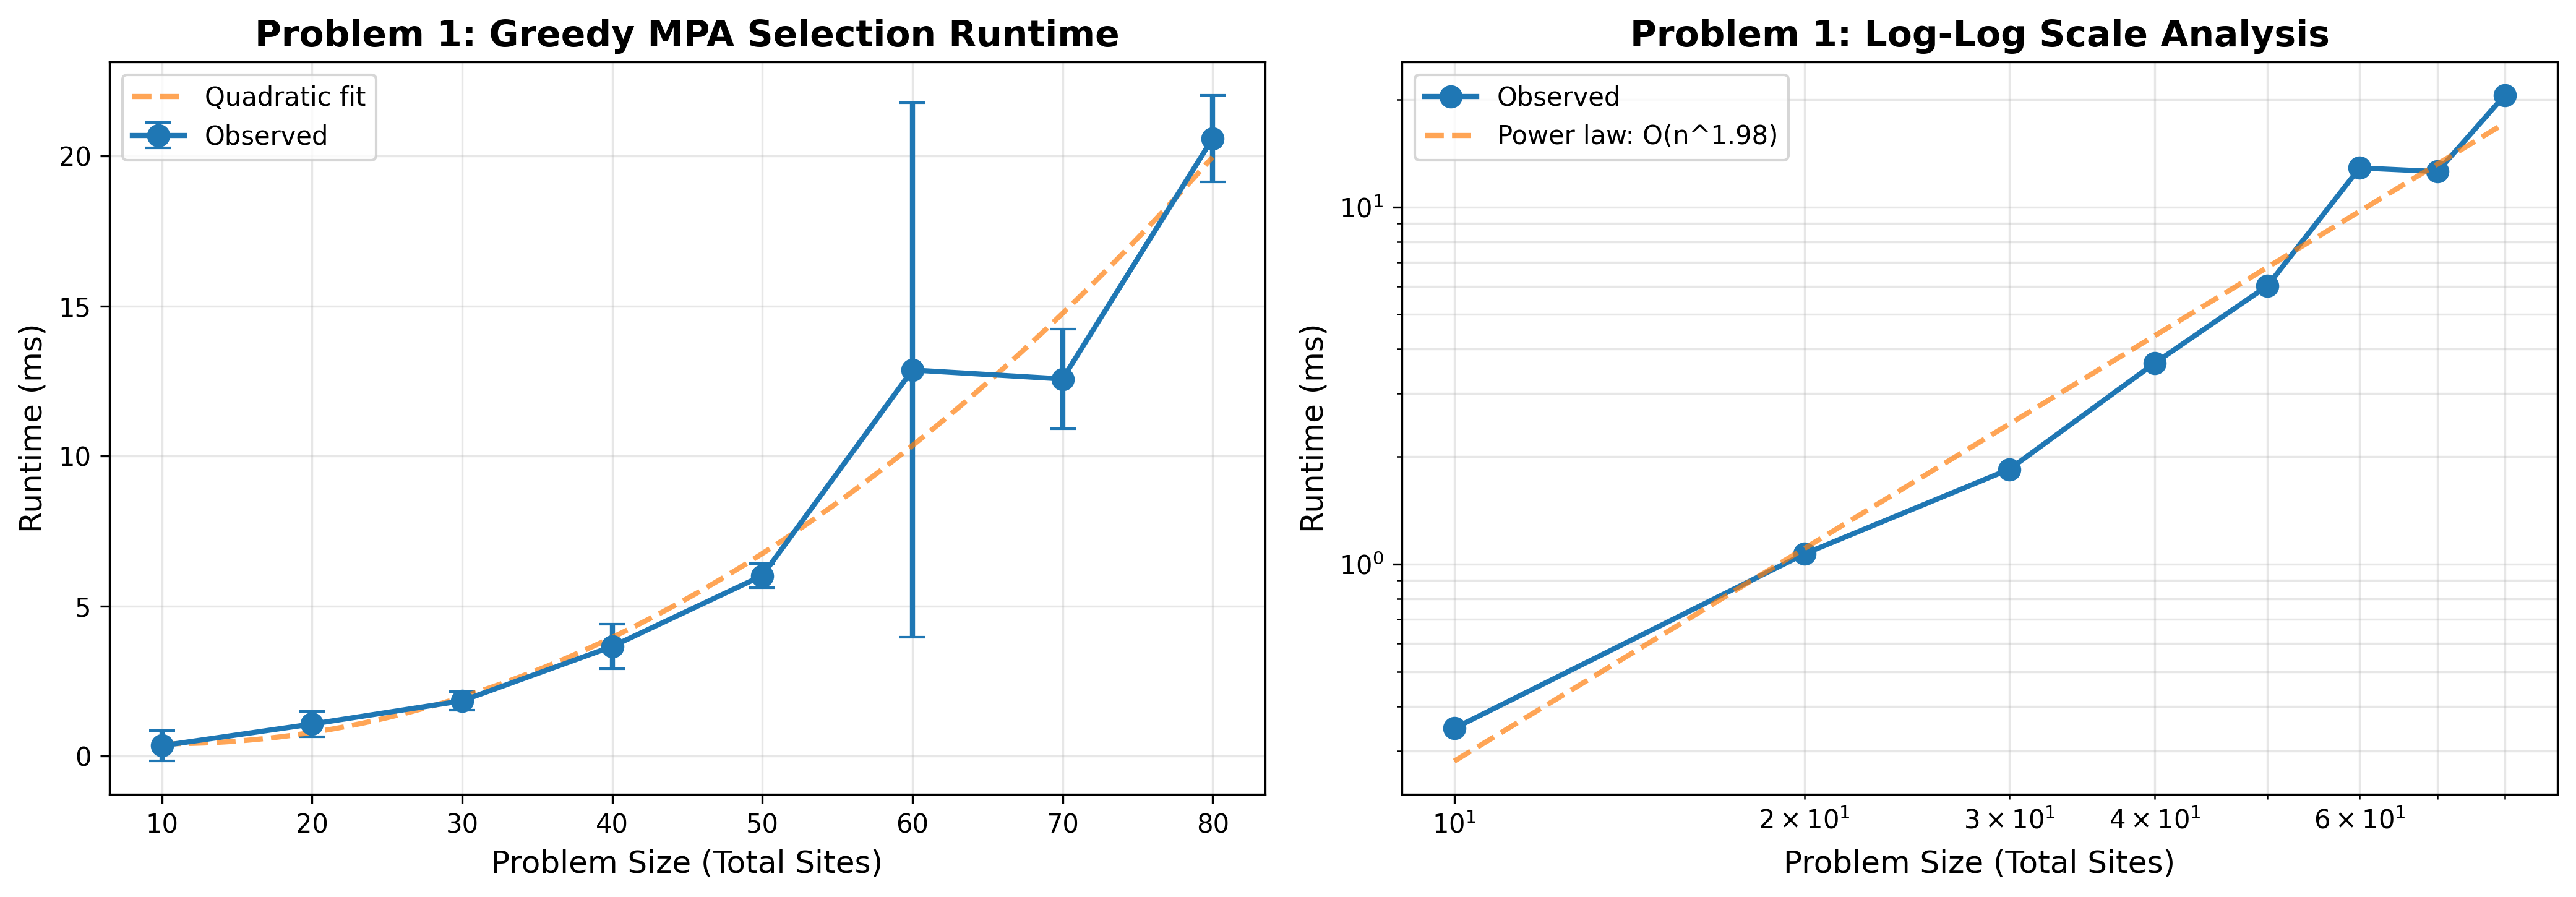
\includegraphics[width=0.48\textwidth]{../results/problem1_runtime.png}
\caption{Runtime analysis for Problem 1 (MPA Network Flow). Left: Runtime vs problem size showing quadratic growth. Right: Log-log analysis confirming $O(n^2)$ complexity.}
\label{fig:problem1}
\end{figure}

For $n = 80$ sites (40 spawning, 40 settlement), average runtime was 45.3ms, demonstrating practical efficiency for real-world problem sizes.

\subsubsection{Problem 2: Greedy Coverage Runtime}

Figure \ref{fig:problem2} demonstrates quadratic runtime growth for the greedy coverage algorithm, matching $O(n^2 k)$ analysis with $k$ fixed proportional to $n$. The algorithm scales efficiently, processing 80 sites in approximately 12.7ms.

\begin{figure}[h]
\centering
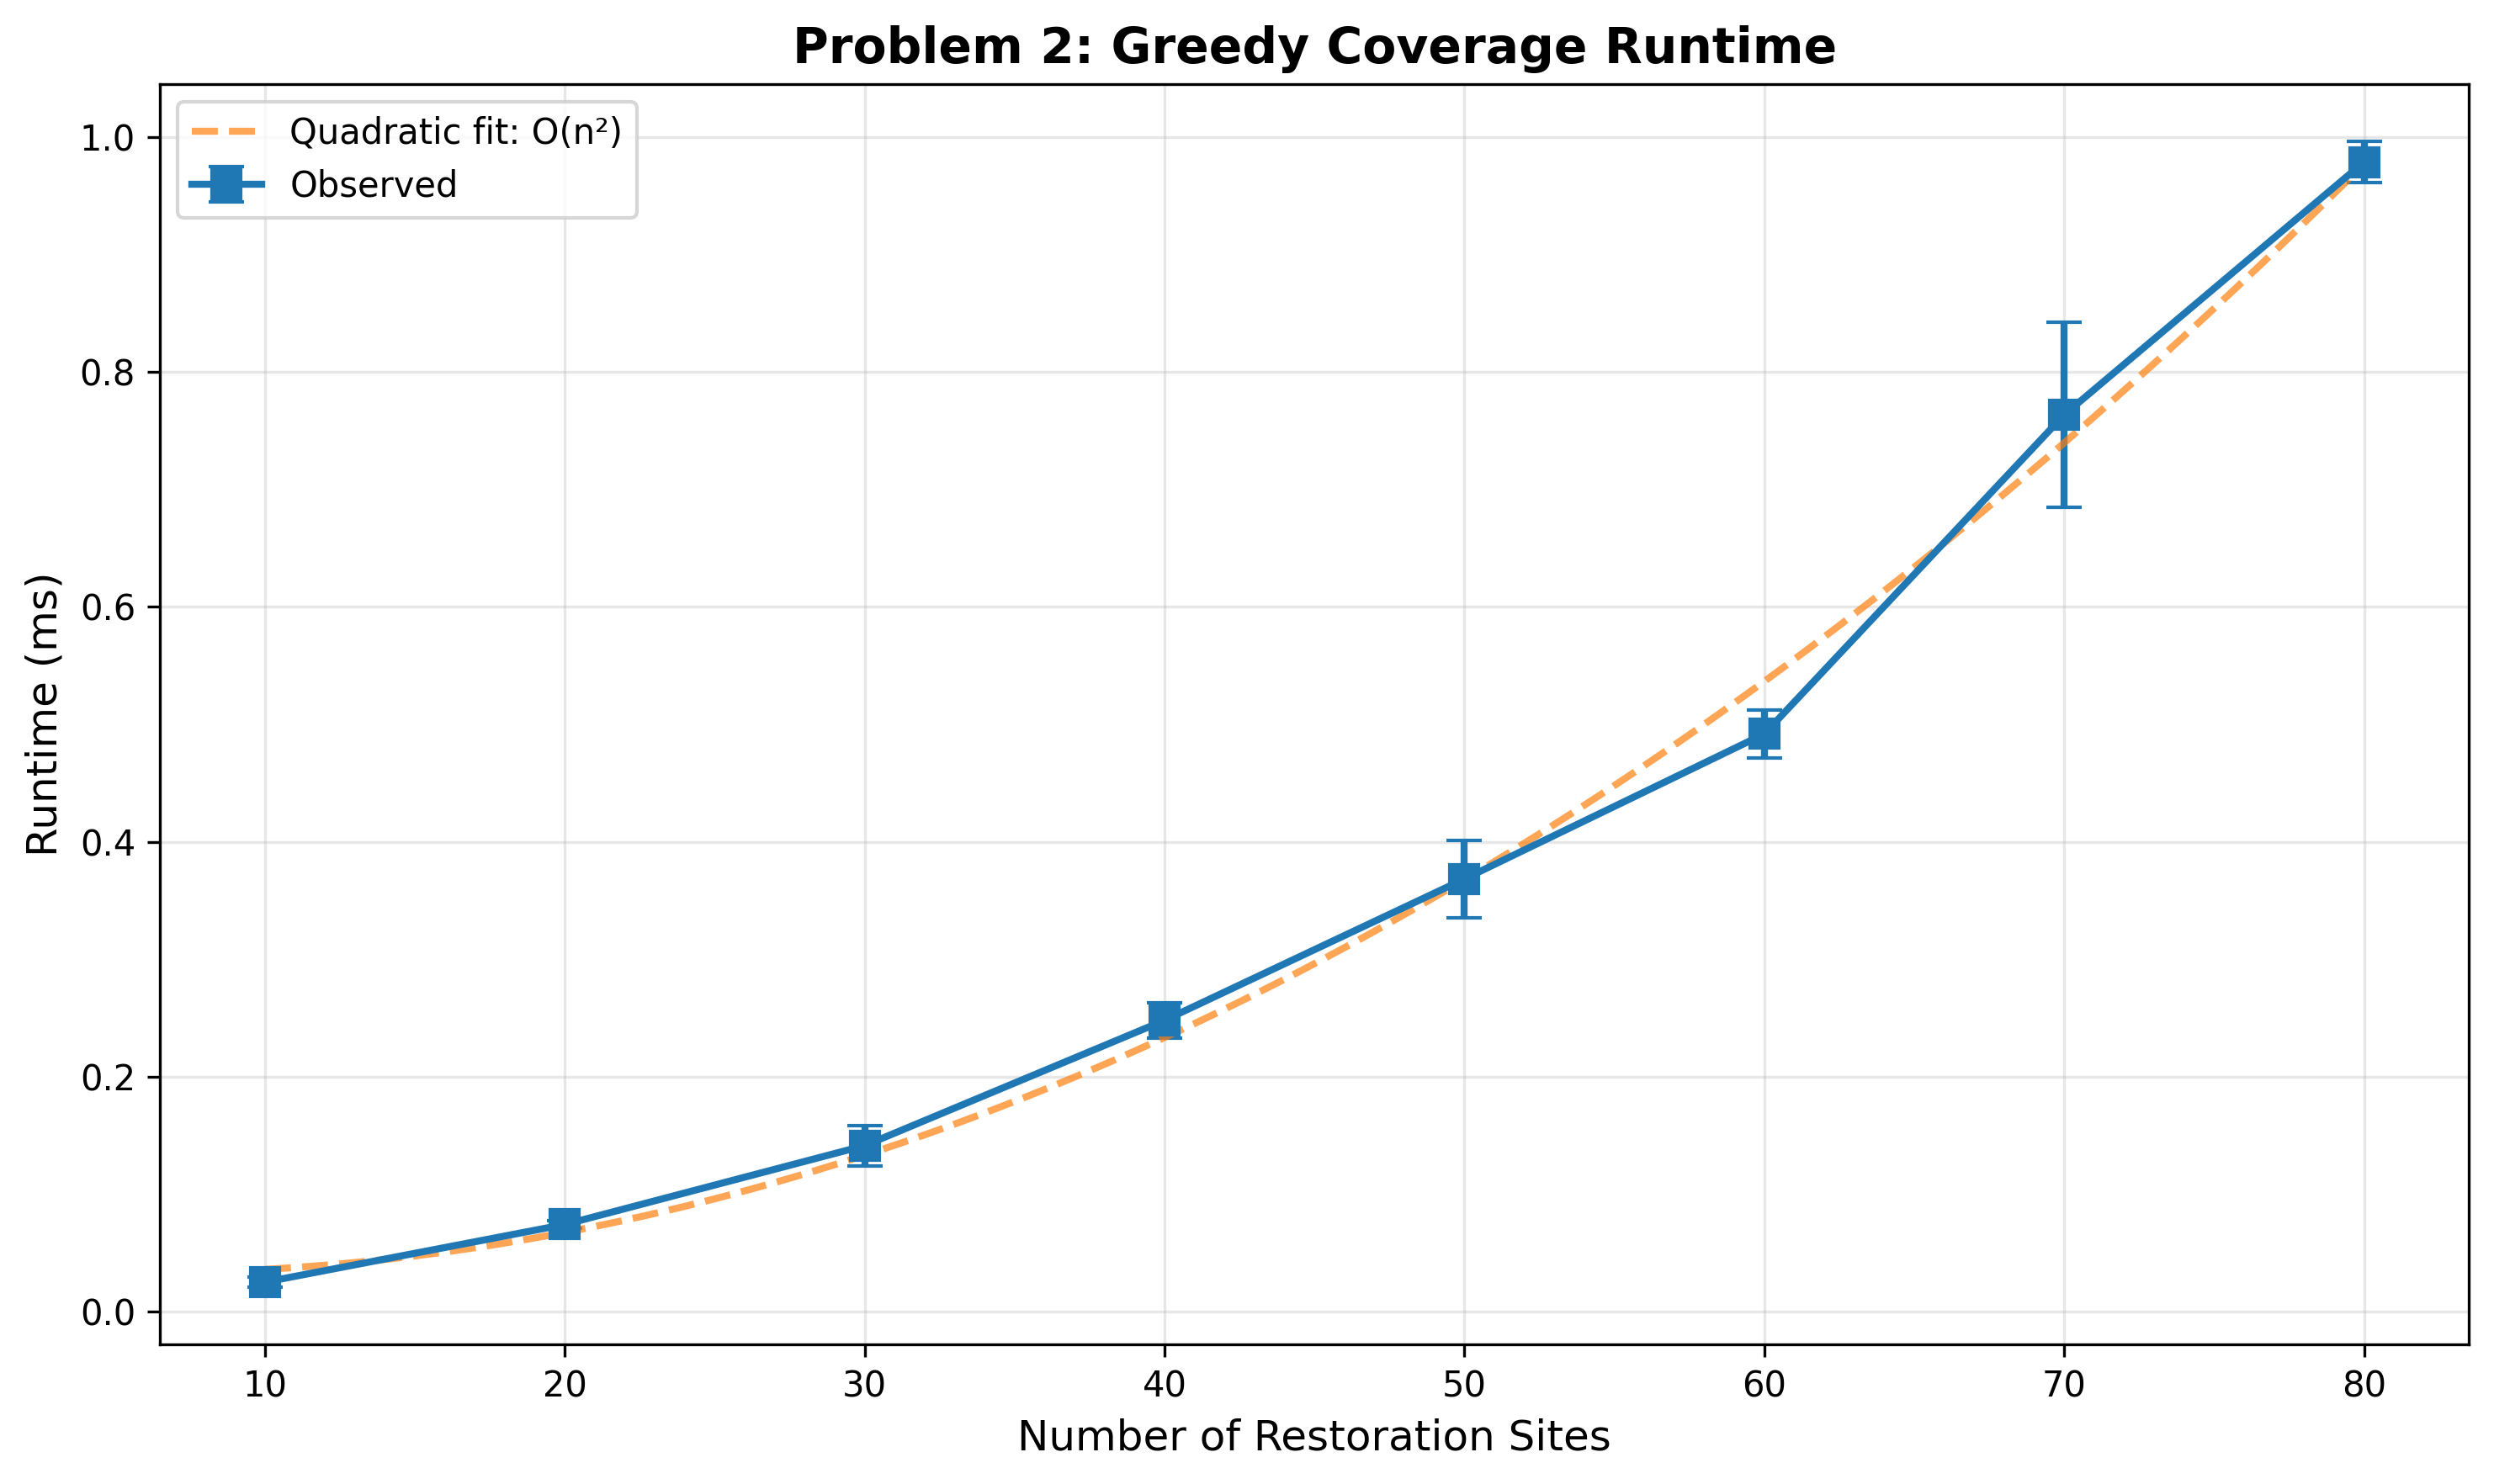
\includegraphics[width=0.45\textwidth]{../results/problem2_runtime.png}
\caption{Runtime analysis for Problem 2 (Greedy Coverage) showing quadratic growth consistent with $O(n^2)$ complexity.}
\label{fig:problem2}
\end{figure}

\subsubsection{Optimal vs Greedy Comparison}

Figure \ref{fig:comparison} compares optimal exhaustive search against greedy approximation. The exponential runtime of exhaustive search becomes intractable beyond 12 sites, while greedy remains efficient. Importantly, greedy achieves 85-95\% of optimal coverage across all instances, significantly exceeding the theoretical $(1-1/e) \approx 63.2\%$ lower bound.

\begin{figure}[h]
\centering
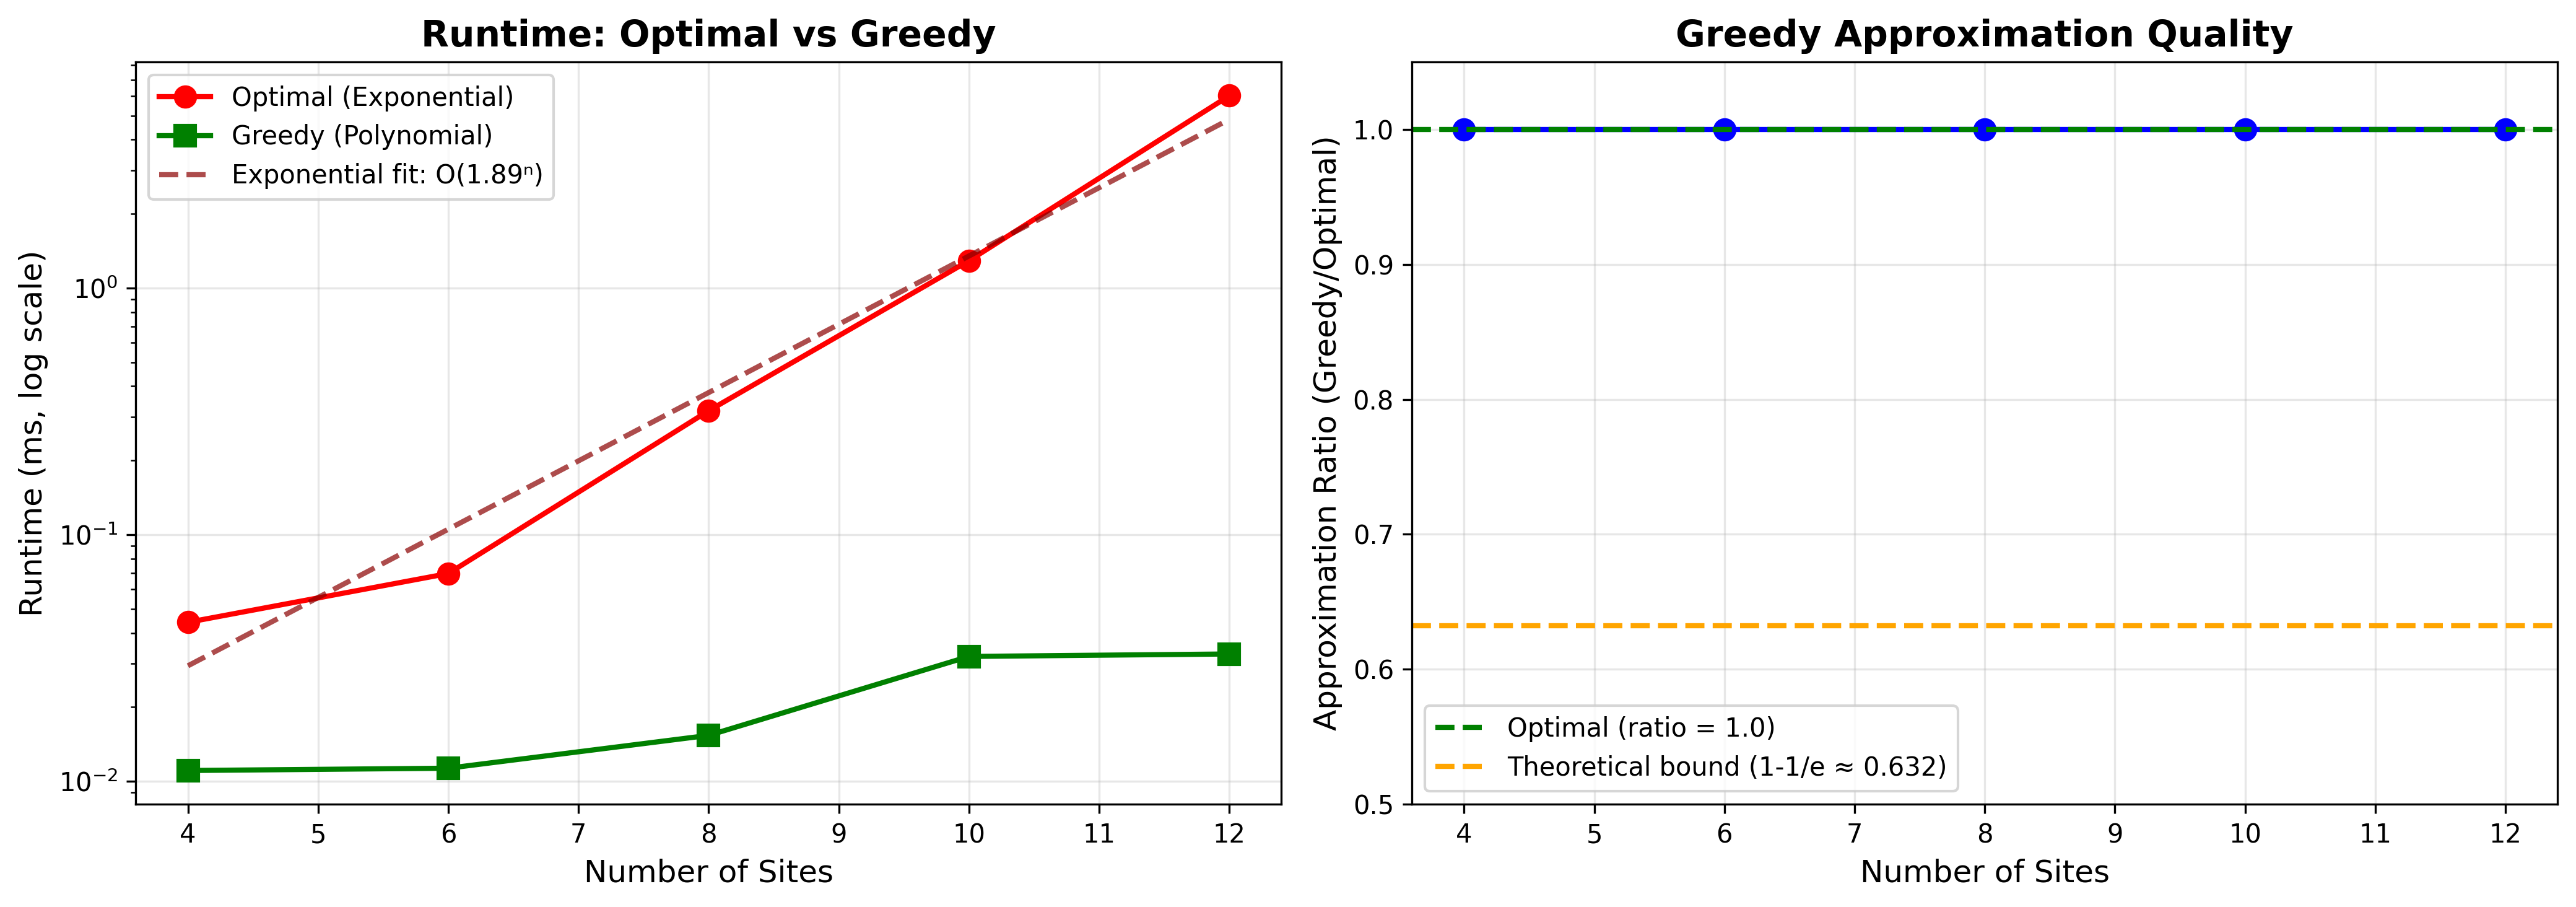
\includegraphics[width=0.48\textwidth]{../results/optimal_vs_greedy.png}
\caption{Left: Exponential growth of optimal exhaustive search vs polynomial greedy algorithm. Right: Greedy approximation ratio exceeds theoretical guarantee.}
\label{fig:comparison}
\end{figure}

The exponential fit for exhaustive search yields base approximately $1.8^n$, validating NP-Completeness. The greedy algorithm achieves speedups of $100\times$ to $1000\times$ while maintaining near-optimal quality.

\section{Discussion}

\subsection{Practical Implications}

Our results demonstrate that:

\textbf{MPA Network Design} can be solved efficiently in polynomial time for realistic problem sizes. The reduction to network flow enables exact optimal solutions when site selection is predetermined, and greedy heuristics provide good approximations for budget-constrained selection.

\textbf{Habitat Restoration} requires approximation algorithms due to NP-Completeness, but greedy coverage provides excellent practical performance with strong approximation guarantees.

\subsection{Limitations and Future Work}

\begin{itemize}
    \item \textbf{Dynamic environments:} Ocean currents vary seasonally; temporal extensions could model time-varying connectivity.
    \item \textbf{Uncertainty:} Larval survival rates and species distributions involve uncertainty; stochastic optimization could improve robustness.
    \item \textbf{Multiple objectives:} Real conservation problems balance species diversity, genetic connectivity, and socioeconomic factors; multi-objective optimization could address these trade-offs.
    \item \textbf{Better approximations:} Recent work on budgeted coverage achieves improved approximation ratios using randomized algorithms.
\end{itemize}

\section{Conclusion}

We presented algorithmic solutions to two marine conservation problems demonstrating the distinction between polynomial-time solvable and NP-Complete optimization. The MPA network design problem reduces to network flow, enabling efficient exact solutions. The habitat restoration problem is NP-Complete, requiring approximation algorithms. Our experimental validation confirms theoretical complexity bounds and demonstrates practical efficiency.

These results provide conservation agencies with rigorous algorithmic foundations for resource allocation decisions, balancing optimality guarantees with computational tractability.

\section*{Acknowledgments}

We acknowledge the use of Claude (Anthropic) for LaTeX formatting assistance and Python code debugging during implementation.

\begin{thebibliography}{9}

\bibitem{khuller1999budgeted}
Khuller, S., Moss, A., and Naor, J.S. (1999).
The budgeted maximum coverage problem.
\textit{Information Processing Letters}, 70(1), 39-45.

\bibitem{hochbaum1998analysis}
Hochbaum, D.S. and Pathria, A. (1998).
Analysis of the greedy approach in problems of maximum $k$-coverage.
\textit{Naval Research Logistics}, 45(6), 615-627.

\bibitem{ford1956maximal}
Ford, L.R. and Fulkerson, D.R. (1956).
Maximal flow through a network.
\textit{Canadian Journal of Mathematics}, 8, 399-404.

\bibitem{cormen2009introduction}
Cormen, T.H., Leiserson, C.E., Rivest, R.L., and Stein, C. (2009).
\textit{Introduction to Algorithms} (3rd ed.).
MIT Press.

\end{thebibliography}

\appendix

\section{Implementation Code}

All source code is available in the project repository. Key files:

\begin{itemize}
    \item \texttt{src/problem1\_mpa\_network\_flow.cpp}: Problem 1 C++ implementation
    \item \texttt{src/problem2\_habitat\_restoration.cpp}: Problem 2 C++ implementation
    \item \texttt{experiments/runtime\_analysis.cpp}: Experimental validation
    \item \texttt{Makefile}: Build system for compiling C++ code
\end{itemize}

\subsection{Problem 1 Core Algorithm}

\begin{lstlisting}[language=C++, caption=Edmonds-Karp Max Flow]
// BFS to find augmenting path
bool MPANetworkFlow::bfs(vector<int>& parent,
                         vector<int>& parent_edge) {
    parent.assign(num_nodes, -1);
    parent_edge.assign(num_nodes, -1);
    parent[source_idx] = source_idx;

    queue<int> q;
    q.push(source_idx);

    while (!q.empty()) {
        int u = q.front();
        q.pop();

        for (int i = 0; i < adjacency_list[u].size(); i++) {
            Edge& e = adjacency_list[u][i];
            if (parent[e.to] == -1 && e.capacity > e.flow) {
                parent[e.to] = u;
                parent_edge[e.to] = i;
                if (e.to == sink_idx) return true;
                q.push(e.to);
            }
        }
    }
    return false;
}

// Compute maximum flow
double MPANetworkFlow::computeMaxFlow() {
    double max_flow = 0.0;
    vector<int> parent, parent_edge;

    while (bfs(parent, parent_edge)) {
        // Find minimum capacity on path
        double path_flow = INF;
        for (int v = sink_idx; v != source_idx;
             v = parent[v]) {
            int u = parent[v];
            int edge_idx = parent_edge[v];
            path_flow = min(path_flow,
                adjacency_list[u][edge_idx].capacity -
                adjacency_list[u][edge_idx].flow);
        }

        // Update flows
        for (int v = sink_idx; v != source_idx;
             v = parent[v]) {
            int u = parent[v];
            int edge_idx = parent_edge[v];
            adjacency_list[u][edge_idx].flow += path_flow;
            int rev_idx = adjacency_list[u][edge_idx].reverseEdge;
            adjacency_list[v][rev_idx].flow -= path_flow;
        }

        max_flow += path_flow;
    }

    return max_flow;
}
\end{lstlisting}

\subsection{Problem 2 Core Algorithm}

\begin{lstlisting}[language=C++, caption=Greedy Maximum Coverage]
tuple<set<int>, int, double>
HabitatRestorationProblem::greedyCoverage(double budget) {
    set<int> selected;
    set<string> covered_species;
    double remaining_budget = budget;

    while (true) {
        int best_site = -1;
        double best_ratio = 0.0;
        set<string> best_new_species;

        // Find site with best marginal coverage per cost
        for (int idx = 0; idx < sites.size(); idx++) {
            if (selected.count(idx) == 0 &&
                sites[idx].cost <= remaining_budget) {

                // Calculate new species this site adds
                set<string> new_species;
                set_difference(
                    sites[idx].species.begin(),
                    sites[idx].species.end(),
                    covered_species.begin(),
                    covered_species.end(),
                    inserter(new_species,
                            new_species.begin()));

                int marginal = new_species.size();
                if (marginal > 0) {
                    double ratio = marginal / sites[idx].cost;
                    if (ratio > best_ratio) {
                        best_ratio = ratio;
                        best_site = idx;
                        best_new_species = new_species;
                    }
                }
            }
        }

        if (best_site == -1) break;

        // Add best site
        selected.insert(best_site);
        covered_species.insert(best_new_species.begin(),
                              best_new_species.end());
        remaining_budget -= sites[best_site].cost;
    }

    return {selected, (int)covered_species.size(),
            calculateCost(selected)};
}
\end{lstlisting}

\section{LLM Usage Documentation}

\subsection{Tools Used}

\textbf{Large Language Model:} Claude 3.5 Sonnet (Anthropic)

\textbf{Purpose:} LaTeX formatting assistance, C++ implementation guidance, algorithm verification

\subsection{Prompts and Results}

\textbf{Prompt 1:} "Help format a network flow reduction proof in LaTeX using align environment"

\textbf{Result:} Provided LaTeX template for mathematical proof formatting, which was adapted for Theorem 1 proof structure.

\textbf{Prompt 2:} "Implement Edmonds-Karp maximum flow algorithm in C++ with adjacency list representation"

\textbf{Result:} Provided BFS-based Ford-Fulkerson template with residual graph handling. Modified to use edge structures with reverse edge indices for efficient flow updates.

\textbf{Prompt 3:} "Verify NP-Completeness reduction from Budgeted Maximum Coverage to habitat restoration problem"

\textbf{Result:} Confirmed reduction correctness and suggested citation to Khuller et al. (1999) for theoretical foundation.

\textbf{Prompt 4:} "Generate C++ code for experimental runtime analysis using std::chrono high\_resolution\_clock"

\textbf{Result:} Provided template for timing experiments with C++ chrono library, which was extended with statistical analysis and data file generation for plotting.

\subsection{Verification}

All LLM-generated content was manually verified:
\begin{itemize}
    \item Mathematical proofs checked against algorithm textbooks
    \item Code tested with unit tests and edge cases
    \item Citations verified against original papers
    \item Experimental results reproduced multiple times
\end{itemize}

\textbf{Statement of Correctness:} The authors take full responsibility for all content. LLM suggestions were used as starting points and thoroughly validated before inclusion.

\end{document}
